\documentclass[a4paper,12pt]{khmermath}
\geometry{left=0.9cm, right=0.9cm, top=0.75cm, bottom=0.85cm, footskip=0.55cm}
\usepackage{pifont}
\usepackage{fancyhdr}

% =========================================================================
% កំណត់ពុម្ពអក្សរ និងពណ៌សោភ័ណភាពបែបសៀវភៅកូរ៉េ (Korean Textbook Palette)
% =========================================================================
\definecolor{koreaTeal}{HTML}{008080}
\definecolor{brandTeal}{HTML}{008282}
\definecolor{brandDarkTeal}{HTML}{004D4D}
\definecolor{brandLightBlue}{HTML}{F4F9FA}
\definecolor{brandTealBg}{HTML}{E8F5F5}
\definecolor{brandNavy}{HTML}{0F2C59}
\definecolor{brandCrimson}{HTML}{C70039}
\definecolor{brandBadgeBg}{HTML}{E8F6F6}
\definecolor{brandGrayText}{HTML}{334155}
\definecolor{brandSoftGray}{HTML}{F8FAFB}
\definecolor{cardBorder}{HTML}{C5E1E1}
\definecolor{koreaPurple}{HTML}{4A55A2}

% =========================================================================
% ក្បាលទំព័រ និងបាតទំព័រ (Header & Footer)
% =========================================================================
\pagestyle{fancy}
\fancyhf{}
\renewcommand{\headrulewidth}{0pt}
\renewcommand{\footrulewidth}{0.6pt}
\renewcommand{\footrule}{\hbox to\headwidth{\color{brandTeal}\leaders\hrule height \footrulewidth\hfill}}

\fancyfoot[L]{\fontsize{8.5}{8.5}\selectfont\color{brandNavy}\textbf{\thepage}\ \textcolor{brandTeal}{|}\ \textbf{\kml\color{brandDarkTeal}\LessonTitle}}
\fancyfoot[C]{\fontsize{8.5}{8.5}\selectfont\color{brandNavy}$\star$ \textbf{\kml បង្រៀនដោយ ៖ ក្រូត រស្មី} $\star$}
\fancyfoot[R]{\fontsize{8.5}{8.5}\selectfont\color{brandNavy}\textbf{Telegram: \textcolor{brandCrimson}{070897540}}\ \textcolor{brandTeal}{|}\ \textbf{\thepage}}

% =========================================================================
% ព័ត៌មានមេរៀន
% =========================================================================
\newcommand{\LessonNum}{01}
\newcommand{\LessonTitle}{ប្រមាណវិធីលើរ៉ាឌីកាល់សន្ទស្សន៍ 2 និង 3}

% =========================================================================
% រចនាប័ទ្មសមាសភាគកូរ៉េ (Korean Components)
% =========================================================================
% ក្បាលចំណងជើងមេរៀន
\newcommand{\koreanheader}[2]{%
  \noindent
  \begin{tikzpicture}[baseline=(num.base)]
    \node[
      fill=brandTeal,
      text=white,
      font=\fontsize{11}{11}\selectfont\kml,
      rounded corners=3.5pt,
      inner xsep=12pt,
      inner ysep=4pt
    ] (num) {មេរៀនទី #1};
    \node[
      anchor=west,
      font=\fontsize{13.5}{13.5}\selectfont\kml,
      text=brandDarkTeal,
      xshift=9pt
    ] (title) at (num.east) {#2};
    \node[
      anchor=east,
      font=\fontsize{8}{8}\selectfont,
      text=gray!75,
      xshift=-2pt
    ] at (\linewidth-0.8cm, 0) {$>$ ក្លឹបសិក្សាគណិតវិទ្យា ភី ស៊ី អឹម};
  \end{tikzpicture}
  \vspace{2pt}
}

% បដាចំណងជើងផ្នែកធំៗ (Section Banner)
\newcommand{\khsection}[2]{%
  \vspace{2pt}\noindent
  \begin{tikzpicture}
    \node[
      fill=brandTealBg,
      rounded corners=3.5pt,
      inner sep=2.8pt,
      text width=\linewidth-5.6pt
    ] {
      \tikz[baseline=(char.base)]{
        \node[fill=brandTeal, text=white, rounded corners=2.5pt, font=\fontsize{8}{8}\selectfont\bfseries, inner sep=2.5pt] (char) {\,#1\,};
      }%
      \hspace{5pt}%
      \fontsize{9.5}{9.5}\selectfont\kml\bfseries\color{brandDarkTeal}#2
    };
  \end{tikzpicture}\par
  \vspace{1.5pt}
}

% លេខលំហាត់ (Exercise Badge)
\newcommand{\koreannum}[1]{%
  \tikz[baseline=(num.base)]{%
    \node[
      fill=brandTeal,
      text=white,
      font=\fontsize{9.5}{9.5}\selectfont\bfseries,
      rounded corners=3pt,
      inner xsep=4.5pt,
      inner ysep=1.8pt
    ] (num) {\ifnum#1<10 0#1\else#1\fi};
  }\ %
}
\newcommand{\exhead}[1]{\noindent\koreannum{#1}}

% អក្សររង ក. ខ. គ...
\newcommand{\subk}[1]{\textcolor{brandCrimson}{\textbf{#1.}}\,}
\newcommand{\circnum}[1]{\tikz[baseline=(n.base)]{\node[circle, fill=brandTeal, text=white, inner sep=1.2pt, font=\fontsize{7.2}{7.2}\selectfont\bfseries] (n) {#1};}\,}

% ម៉ាក្រូបង្ហាញគំរូដំណោះស្រាយតាមប្រភេទលំហាត់នីមួយៗ (Expanded & Clear Worked Example Model)
\newcommand{\khmodel}[1]{%
  \par\vspace{1.2pt}%
  \noindent\colorbox{brandTealBg!55}{%
    \parbox{\linewidth-6pt}{%
      \fontsize{8.5}{11.5}\selectfont\color{brandDarkTeal}%
      \textbf{\textcolor{brandCrimson}{\ding{229}}\ \kml គំរូ ៖} #1%
    }%
  }\par\vspace{1.5pt}%
}

% Macros សម្រាប់តម្រឹមធាតុឱ្យមានរបៀប និងជួរឈរស្មើគ្នា (Clean Column Grid)
\newcommand{\coltwo}[2]{%
  \noindent\makebox[0.5\linewidth][l]{#1}\makebox[0.5\linewidth][l]{#2}\par\vspace{1pt}%
}
\newcommand{\colthree}[3]{%
  \noindent\makebox[0.333\linewidth][l]{#1}\makebox[0.333\linewidth][l]{#2}\makebox[0.333\linewidth][l]{#3}\par\vspace{1pt}%
}
\newcommand{\colfour}[4]{%
  \noindent\makebox[0.25\linewidth][l]{#1}\makebox[0.25\linewidth][l]{#2}\makebox[0.25\linewidth][l]{#3}\makebox[0.25\linewidth][l]{#4}\par\vspace{1pt}%
}
\newcommand{\colfive}[5]{%
  \noindent\makebox[0.2\linewidth][l]{#1}\makebox[0.2\linewidth][l]{#2}\makebox[0.2\linewidth][l]{#3}\makebox[0.2\linewidth][l]{#4}\makebox[0.2\linewidth][l]{#5}\par\vspace{1pt}%
}

% -------------------------------------------------------------------------
% ប្រអប់ទ្រឹស្តី (Theory Box)
% -------------------------------------------------------------------------
\newtcolorbox{theorybox}[1][]{
  enhanced,
  colframe=brandNavy!45,
  colback=brandLightBlue,
  boxrule=0.7pt,
  arc=3.5pt,
  borderline west={3pt}{0pt}{koreaTeal},
  drop fuzzy shadow=brandNavy!12,
  left=7pt, right=7pt, top=4pt, bottom=3pt,
  title={\fontsize{9.2}{9.2}\selectfont\kml\color{white}\ding{72}\ រំលឹកទ្រឹស្តី និងរូបមន្តគន្លឹះសំខាន់ៗ},
  coltitle=white,
  colbacktitle=brandNavy,
  boxed title style={
    boxrule=0pt,
    arc=2.5pt,
    left=6pt, right=6pt, top=1.5pt, bottom=1.5pt
  },
  attach boxed title to top left={yshift*=-\tcboxedtitleheight/2, xshift=9pt},
  #1
}

\setlength{\columnsep}{15pt}
\setlength{\parindent}{0pt}
\setlength{\parskip}{0.6pt}
\everymath{\displaystyle}
\DeclareMathSizes{12pt}{13pt}{11pt}{10pt}
\DeclareMathSizes{10pt}{11pt}{9pt}{8pt}

% =========================================================================
% ចាប់ផ្តើមតួខ្លឹមសារឯកសារ (DOCUMENT CONTENT)
% =========================================================================
\begin{document}

% -------------------------------------------------------------------------
% ទំព័រទី ១ ៖ មេរៀនទី ១, ទ្រឹស្តី និង ផ្នែកទី ១ (គណនាឬសការេ និងឬសគូប)
% -------------------------------------------------------------------------

% ១. បដាក្បាលទំព័រមេរៀន
\koreanheader{\LessonNum}{\LessonTitle}

% ២. ប្រអប់ទ្រឹស្តីសង្ខេប
\begin{theorybox}
  \begin{enumerate}[label=\protect\circnum{\arabic*}, leftmargin=15pt, itemsep=0.4pt, topsep=0pt]
    \item \textbf{និយមន័យ ៖} បើ $a > 0,\, x^2 = a \implies x = \pm\sqrt{a}$ \quad $|$ \quad បើ $x^3 = a \implies x = \sqrt[3]{a}$ ដែល $a \in \mathbb{R}$ ។
    \item \textbf{លក្ខណៈសំខាន់ ($a, b > 0, b \neq 0$) ៖}
      $\sqrt{a}\cdot\sqrt{b} = \sqrt{ab}$ , \quad $\sqrt[3]{a}\cdot\sqrt[3]{b} = \sqrt[3]{ab}$ , \quad $\frac{\sqrt{a}}{\sqrt{b}} = \sqrt{\frac{a}{b}}$ , \quad $\frac{\sqrt[3]{a}}{\sqrt[3]{b}} = \sqrt[3]{\frac{a}{b}}$ ។
    \item \textbf{វិធីបូក-ដករ៉ាឌីកាល់ ៖} ត្រូវបម្លែងឱ្យសន្ទស្សន៍ និងរ៉ាឌីកង់ដូចគ្នា រួចបូកឬដកតែមេគុណ ។
    \item \textbf{បំបាត់រ៉ាឌីកាល់ពីភាគបែង ៖}
    \begin{itemize}[leftmargin=11pt, itemsep=0.3pt, topsep=0pt, label=\color{brandCrimson}\ding{226}]
      \item $(a-b)(a+b)=a^2-b^2$ \quad និង \quad $a^3 \pm b^3 = (a \pm b)(a^2 \mp ab + b^2)$
      \item \textit{ភាគបែងជាឬសការេ ៖} $\frac{1}{\sqrt{7}-1} = \frac{\sqrt{7}+1}{(\sqrt{7}-1)(\sqrt{7}+1)} = \frac{\sqrt{7}+1}{7-1} = \frac{\sqrt{7}+1}{6}$
      \item \textit{ភាគបែងជាឬសគូប ៖} $\frac{1}{\sqrt[3]{2}+1} = \frac{\sqrt[3]{4}-\sqrt[3]{2}+1}{(\sqrt[3]{2}+1)(\sqrt[3]{4}-\sqrt[3]{2}+1)} = \frac{\sqrt[3]{4}-\sqrt[3]{2}+1}{3}$
    \end{itemize}
  \end{enumerate}
\end{theorybox}

\vspace{1pt}

\setlength{\columnseprule}{0.4pt}
\def\columnseprulecolor{\color{cardBorder}}

\begin{multicols}{2}

  % =======================================================================
  % ផ្នែកទី ១ ៖ គណនាឬសការេ និងឬសគូប
  % =======================================================================
  \khsection{I}{គណនាឬសការេ និងឬសគូប}

  % --- លំហាត់ ០១ ---
  \exhead{1} \textbf{គណនា ៖}\par
  \khmodel{%
    \subk{ក} $\sqrt{9} = 3$ \quad
    \subk{ឈ} $\sqrt[3]{8} = 2$ \quad
    \subk{ត} $\sqrt{\tfrac{9}{16}} = \tfrac{3}{4}$ \quad
    \subk{ផ} $\sqrt[3]{\tfrac{1}{8}} = \tfrac{1}{2}$%
  }
  \colfour{\subk{ក} $\sqrt{9}$}{\subk{ខ} $\sqrt{16}$}{\subk{គ} $\sqrt{36}$}{\subk{ឃ} $-\sqrt{64}$}
  \colfour{\subk{ង} $-\sqrt{100}$}{\subk{ច} $\sqrt{121}$}{\subk{ឆ} $-\sqrt{144}$}{\subk{ជ} $\sqrt{625}$}
  \colthree{\subk{ឈ} $\sqrt[3]{8}$}{\subk{ញ} $\sqrt[3]{-8}$}{\subk{ដ} $-\sqrt[3]{27}$}
  \colthree{\subk{ឋ} $-\sqrt[3]{64}$}{\subk{ឌ} $\sqrt[3]{125}$}{\subk{ឍ} $\sqrt[3]{216}$}
  \colthree{\subk{ណ} $\sqrt[3]{1000}$}{\subk{ត} $\sqrt{\tfrac{9}{16}}$}{\subk{ថ} $\sqrt{\tfrac{49}{9}}$}
  \colthree{\subk{ទ} $-\sqrt{\tfrac{81}{4}}$}{\subk{ធ} $\sqrt{\tfrac{169}{49}}$}{\subk{ន} $\sqrt{\tfrac{196}{25}}$}
  \colthree{\subk{ប} $-\sqrt{\tfrac{400}{225}}$}{\subk{ផ} $\sqrt[3]{\tfrac{1}{8}}$}{\subk{ព} $\sqrt[3]{\tfrac{8}{27}}$}
  \coltwo{\subk{ភ} $\sqrt[3]{\tfrac{64}{125}}$}{\subk{ម} $\sqrt[3]{\tfrac{512}{343}}$}

  \vspace{2pt}
  % --- លំហាត់ ០២ ---
  \exhead{2} \textbf{សម្រួលរ៉ាឌីកាល់ ៖}\par
  \khmodel{%
    \subk{ខ} $(\sqrt[3]{-8})^3 = -8$ \quad
    \subk{ឃ} $\sqrt[3]{8^2} = 2^2 = 4$ \quad
    \subk{ទ} $\sqrt{x^2 y^4} = |x| y^2$%
  }
  \colthree{\subk{ក} $\sqrt[3]{1^5}$}{\subk{ខ} $(\sqrt[3]{-8})^3$}{\subk{គ} $\sqrt[3]{(-27)^3}$}
  \colthree{\subk{ឃ} $\sqrt[3]{8^2}$}{\subk{ង} $\sqrt[3]{(-27)^2}$}{\subk{ច} $\sqrt[3]{64^2}$}
  \colthree{\subk{ឆ} $\sqrt{16^3}$}{\subk{ជ} $\sqrt{25^3}$}{\subk{ឈ} $\sqrt{64^3}$}
  \colthree{\subk{ញ} $-\sqrt[3]{36^2}$}{\subk{ដ} $\sqrt{y^2}$}{\subk{ឋ} $\sqrt[3]{x^3}$}
  \colthree{\subk{ឌ} $\sqrt{x^4}$}{\subk{ឍ} $\sqrt[3]{y^6}$}{\subk{ណ} $\sqrt{y^6}$}
  \colthree{\subk{ត} $\sqrt{25a^2}$}{\subk{ថ} $\sqrt[3]{-8b^3}$}{\subk{ទ} $\sqrt{x^2 y^4}$}
  \colthree{\subk{ធ} $\sqrt{36a^4 b^6}$}{\subk{ន} $\sqrt{\tfrac{16}{x^2}}$}{\subk{ប} $\sqrt[3]{\tfrac{27}{y^3}}$}
  \coltwo{\subk{ផ} $\sqrt{\tfrac{100}{n^4}}$}{\subk{ព} $\sqrt{\tfrac{49a^2}{81b^4}}$}

  \columnbreak

  % --- លំហាត់ ០៣ ---
  \exhead{3} \textbf{សម្រួលកន្សោម ៖}\par
  \khmodel{%
    \subk{ក} $\sqrt{(2x)^2} = 2x$ \quad
    \subk{ខ} $\sqrt[3]{(-5y)^3} = -5y$ \quad
    \subk{ង} $\sqrt{(4b+3)^2} = |4b+3|$%
  }
  \coltwo{\subk{ក} $\sqrt{(2x)^2}$}{\subk{ខ} $\sqrt[3]{(-5y)^3}$}
  \coltwo{\subk{គ} $\sqrt{(4 - a)^2}$}{\subk{ឃ} $\sqrt[3]{(x + 3)^3}$}
  \subk{ង} $\sqrt{16b^2 + 24b + 9}$\par\vspace{1pt}
  \subk{ច} $\sqrt{9x^2 - 30x + 25}$\par\vspace{1pt}
  \subk{ឆ} $\sqrt{4m^2 - 20mn + 25n^2}$\par\vspace{1pt}
  \subk{ជ} $\sqrt{49x^2 - 112xy + 64y^2}$

  \vspace{2.5pt}
  % --- លំហាត់ ០៤ ---
  \exhead{4} \textbf{សម្រួលកន្សោមប្រភាគ ៖}\par
  \khmodel{$A = \sqrt{\tfrac{b^2}{(b-7)^2}} = \left|\tfrac{b}{b-7}\right|$}
  \coltwo{$A = \sqrt{\tfrac{b^2}{b^2 - 14b + 49}}$}{$B = \sqrt{\tfrac{49x^2 - 56x + 16}{36x^2}}$}
  \coltwo{$C = \sqrt{\tfrac{a^2 + 16ab + 64b^2}{a^2 + 10ab + 25b^2}}$}{$D = \sqrt{\tfrac{25b^2 + 10ab + a^2}{16b^2 + 24ab + 9a^2}}$}

  \vspace{2.5pt}
  % --- លំហាត់ ០៥ ---
  \exhead{5} \textbf{សម្រួលកន្សោមរ៉ាឌីកាល់ឌុប ៖}\par
  \khmodel{%
    $A = \sqrt{22-12\sqrt{2}} = 3\sqrt{2}-2$ \quad
    $B = \sqrt{(2-\sqrt{3})^2} = 2-\sqrt{3}$%
  }
  \coltwo{$A = \sqrt{22 - \sqrt{288}}$}{$B = \sqrt{7 - 2\sqrt{12}}$}
  \coltwo{$C = \sqrt{9 + \sqrt{32}}$}{$D = \sqrt{13 - \sqrt{48}}$}
  \coltwo{$E = \sqrt{3 + \sqrt{5}}$}{$F = \sqrt{6 + \sqrt{11}}$}

  \vspace{2pt}
  % --- លំហាត់ ០៦ ---
  \exhead{6} \textbf{ប្រៀបធៀបចំនួន} $\sqrt{2}$ និង $\sqrt[3]{3}$ ៖\par
  \khmodel{លើកជាស្វ័យគុណ $6$ ៖ $(\sqrt{2})^6 = 2^3 = 8 < (\sqrt[3]{3})^6 = 3^2 = 9 \implies \sqrt{2} < \sqrt[3]{3}$}
  \vspace{1pt}

\end{multicols}

\newpage

% -------------------------------------------------------------------------
% ទំព័រទី ២ ៖ ផ្នែកទី ២ និង ផ្នែកទី ៣ (ផ្នែកបូក-ដក)
% -------------------------------------------------------------------------
\begin{multicols}{2}

  % =======================================================================
  % ផ្នែកទី ២ ៖ បញ្ចេញ និងបញ្ចូលមួយចំនួនពីរ៉ាឌីកាល់
  % =======================================================================
  \khsection{II}{បញ្ចេញ និងបញ្ចូលមួយចំនួនពីរ៉ាឌីកាល់}

  % --- លំហាត់ ០៧ ---
  \exhead{7} \textbf{បញ្ចេញមួយចំនួនពីរ៉ាឌីកាល់ ៖}\par
  \khmodel{%
    \subk{ក} $\sqrt{18} = 3\sqrt{2}$ \quad
    \subk{ច} $\sqrt[3]{40} = 2\sqrt[3]{5}$ \quad
    \subk{ឋ} $\sqrt{36a^2 b^3} = 6|a|b\sqrt{b}$%
  }
  \colfour{\subk{ក} $\sqrt{18}$}{\subk{ខ} $-\sqrt{48}$}{\subk{គ} $\sqrt{75}$}{\subk{ឃ} $\sqrt{\tfrac{30}{49}}$}
  \colfour{\subk{ង} $\sqrt{\tfrac{10}{121}}$}{\subk{ច} $\sqrt[3]{40}$}{\subk{ឆ} $\sqrt[3]{54}$}{\subk{ជ} $-\sqrt[3]{128}$}
  \coltwo{\subk{ឈ} $\sqrt[3]{192}$}{\subk{ញ} $\sqrt[3]{\tfrac{3m}{8n^3}}$}
  \coltwo{\subk{ដ} $\sqrt[3]{16a^5}$}{\subk{ឋ} $\sqrt{36a^2 b^3}$}
  \coltwo{\subk{ឌ} $\sqrt{27a^4 b^3}$}{\subk{ឍ} $\sqrt{72x^5 y^2}$}
  \coltwo{\subk{ណ} $\sqrt{80m^4 n^3}$}{\subk{ត} $-\sqrt{112a^3 b^4}$}
  \coltwo{\subk{ថ} $\sqrt{64x^2 y^3}$}{\subk{ទ} $\sqrt[3]{16m^3 n^3}$}
  \coltwo{\subk{ធ} $\sqrt[3]{-54x^4 b^3}$}{\subk{ន} $-\sqrt[3]{128a^5 y^3}$}

  \vspace{2pt}
  \vspace{4pt}
  % --- លំហាត់ ០៨ ---
  \exhead{8} \textbf{បញ្ចូលមួយចំនួនក្នុងរ៉ាឌីកាល់} ($x, y, m, n, p > 0$) ៖\par
  \khmodel{%
    \subk{ក} $5\sqrt{6} = \sqrt{5^2 \times 6} = \sqrt{150}$ \quad
    \subk{ឃ} $2\sqrt[3]{5} = \sqrt[3]{2^3 \times 5} = \sqrt[3]{40}$%
  }
  \colthree{\subk{ក} $5\sqrt{6}$}{\subk{ខ} $2m\sqrt{m}$}{\subk{គ} $\tfrac{\sqrt{23}}{y^3}$}
  \colthree{\subk{ឃ} $2\sqrt[3]{5}$}{\subk{ង} $2x\sqrt[3]{4}$}{\subk{ច} $\sqrt[3]{\tfrac{3m}{2n}}$}

  \vspace{2.5pt}
  % =======================================================================
  % ផ្នែកទី ៣ ៖ ប្រមាណវិធីលើរ៉ាឌីកាល់ (បូក ដក គុណ)
  % =======================================================================space{4pt}
  \khsection{III}{ប្រមាណវិធីលើរ៉ាឌីកាល់ (បូក ដក គុណ)}

  % --- លំហាត់ ០៩ ---
  \exhead{9} \textbf{គណនា ៖}\par
  \khmodel{%
    \subk{ក} $(3 - 4 + 5 - 3)\sqrt{2} = \sqrt{2}$ \quad
    \subk{ង} $3\sqrt[3]{2} - 5\sqrt[3]{3}$%
  }
  \subk{ក} $3\sqrt{2} - 4\sqrt{2} + 5\sqrt{2} - 3\sqrt{2}$\par\vspace{1pt}
  \subk{ខ} $5\sqrt{2} - 3\sqrt{3} - 6\sqrt{2} + 5\sqrt{3}$\par\vspace{1pt}
  \subk{គ} $3\sqrt{15} - 4\sqrt{3} - 3\sqrt{15} + 6\sqrt{3}$\par\vspace{1pt}
  \subk{ឃ} $4\sqrt{3} - 2\sqrt{17} + 3\sqrt{17} - 3\sqrt{3} - 2\sqrt{3}$\par\vspace{1pt}
  \subk{ង} $2\sqrt[3]{2} - 8\sqrt[3]{3} + \sqrt[3]{2} + 3\sqrt[3]{3}$\par\vspace{1pt}
  \subk{ច} $8\sqrt[3]{2} - 3\sqrt[3]{3} - 5\sqrt[3]{2} + 2\sqrt[3]{3}$

  \vspace{3pt}
  % --- លំហាត់ ១០ ---
  \exhead{10} \textbf{គណនា ៖}\par
  \khmodel{%
    \subk{ក} $\tfrac{2}{3}(3\sqrt{3}) - \tfrac{3}{4}(4\sqrt{3}) = -\sqrt{3}$ \quad
    \subk{ឃ} $20\sqrt[3]{2} - 15\sqrt[3]{2} = 5\sqrt[3]{2}$%
  }
  \coltwo{\subk{ក} $\tfrac{2}{3}\sqrt{27} - \tfrac{3}{4}\sqrt{48}$}{\subk{ខ} $\tfrac{1}{4}\sqrt{288} - \tfrac{1}{6}\sqrt{72}$}
  \coltwo{\subk{គ} $\tfrac{3}{5}\sqrt{75} - \tfrac{2}{3}\sqrt{27}$}{\subk{ឃ} $5\sqrt[3]{128} - 3\sqrt[3]{250}$}
  \coltwo{\subk{ង} $3\sqrt[3]{81} - \tfrac{1}{2}\sqrt[3]{192}$}{\subk{ច} $4\sqrt[3]{54} - 3\sqrt[3]{128}$}

  \vspace{3pt}
  % --- លំហាត់ ១១ ---
  \exhead{11} \textbf{គណនា ៖}\par
  \khmodel{%
    \subk{ក} $4\sqrt{2} - 21\sqrt{2} - 20\sqrt{2} = -37\sqrt{2}$ \quad
    \subk{ង} $5\sqrt[3]{2}$%
  }
  \subk{ក} $2\sqrt{8} - 3\sqrt{98} - 2\sqrt{200}$\par\vspace{1pt}
  \subk{ខ} $-3\sqrt{50} - \sqrt{32} + 5\sqrt{200}$\par\vspace{1pt}
  \subk{គ} $3\sqrt{175} - 2\sqrt{28} + 3\sqrt{63} - \sqrt{112}$\par\vspace{1pt}
  \subk{ឃ} $\sqrt{108} - 2\sqrt{27} - \sqrt{40} - 5\sqrt{160}$\par\vspace{1pt}
  \subk{ង} $2\sqrt[3]{16} + 3\sqrt[3]{54} - 2\sqrt[3]{128}$\par\vspace{1pt}
  \subk{ច} $3\sqrt[3]{81} + \tfrac{1}{2}\sqrt[3]{128} - 3\sqrt[3]{192} + 4\sqrt[3]{54}$\par\vspace{1pt}
  \subk{ឆ} $4\sqrt[3]{54} - 6\sqrt[3]{81} - 4\sqrt[3]{16} + 3\sqrt[3]{24}$\par\vspace{1pt}
  \subk{ជ} $-2\sqrt[3]{40} - 3\sqrt[3]{135} + 5\sqrt[3]{320} + 8\sqrt[3]{5}$

  \vspace{2.5pt}
  \columnbreak

% --- លំហាត់ ១២ ---
  \exhead{12} \textbf{គណនា ៖}\par
  \khmodel{%
    \subk{ក} $-4\sqrt{12}+2\sqrt{18}-15\sqrt{32}+5\sqrt{27} = 7\sqrt{3}-54\sqrt{2}$%
  }
  \subk{ក} $-2(2\sqrt{12} - \sqrt{18}) - 5(3\sqrt{32} - \sqrt{27})$\par\vspace{1pt}
  \subk{ខ} $3(3\sqrt[3]{40} - \sqrt[3]{135}) + 4(\sqrt[3]{320} - \sqrt[3]{40})$\par\vspace{1pt}
  \subk{គ} $\tfrac{2\sqrt{27}}{3} - 3\sqrt{48} + \tfrac{4\sqrt{50}}{5} - \tfrac{4\sqrt{18}}{3}$\par\vspace{1pt}
  \subk{ឃ} $\tfrac{2}{3}\sqrt[3]{81} - \tfrac{1}{2}\sqrt[3]{24} + \tfrac{2\sqrt[3]{135}}{3} - \tfrac{3\sqrt[3]{40}}{2}$



% -------------------------------------------------------------------------
% -------------------------------------------------------------------------

  % --- លំហាត់ ១៣ ---
  \exhead{13} \textbf{គណនាកន្សោមខាងក្រោម} ($a, b, x, y, z > 0$) ៖\par
  \khmodel{%
    $A = -12\sqrt{2x} + 12\sqrt{2x} = 0$ \quad
    $G = 36a\sqrt[3]{2a}$%
  }
  $A = -3\sqrt{32x} + 6\sqrt{8x}$\par\vspace{1pt}
  $B = 2\sqrt{125x^2 z} + 8x\sqrt{80z}$\par\vspace{1pt}
  $C = 7a\sqrt{b^3} + b\sqrt{4a^2 b} - \sqrt{4b}$\par\vspace{1pt}
  $D = 8b\sqrt{49b} - 7\sqrt{9b^3} + a\sqrt{4a} + \sqrt{a^3}$\par\vspace{1pt}
  $E = 3xy\sqrt{x^2 y} - 2\sqrt{x^4 y^3}$\par\vspace{1pt}
  $F = -3a\sqrt{a^3 b^5} - 2b\sqrt{a^5 b^3} + 5\sqrt{a^5 b^3}$\par\vspace{1pt}
  $G = 8a\sqrt[3]{54a} + 6\sqrt[3]{16a^4}$\par\vspace{1pt}
  $H = 3\sqrt[3]{x^4 y} - 6x\sqrt[3]{xy^4} + 2\sqrt[3]{x^4 y^4}$

  \vspace{2.5pt}
  % --- លំហាត់ ១៤ ---
  \exhead{14} \textbf{គណនាតម្លៃលេខនៃកន្សោម ៖}\par
  \khmodel{\circnum{1} ជំនួស $a=5, b=3$ ៖ $A = \sqrt{15}-3\sqrt{15}-45\sqrt{15}-5\sqrt{15} = -52\sqrt{15}$}
  \circnum{1} $A = \sqrt{ab} - \sqrt{ab^3} - \sqrt{9a^3 b^3} - \sqrt{a^3 b}$ \quad ចំពោះ $a = 5, b = 3$\par\vspace{1pt}
  \circnum{2} $A = \sqrt{4a} + a\sqrt{a^2 b} + \sqrt{b^2 a} + b\sqrt{9b}$ \quad ចំពោះ $a = 3, b = 2$

  \vspace{2.5pt}
  % --- លំហាត់ ១៥ ---
  \exhead{15} \textbf{គណនា ៖}\par
  \khmodel{%
    \subk{ក} $6\sqrt{6}$ \quad
    \subk{ជ} $15\sqrt[3]{30}$ \quad
    \subk{ញ} $3\sqrt{5}(6\sqrt{2} - 12\sqrt{3}) = 18\sqrt{10} - 36\sqrt{15}$%
  }
  \coltwo{\subk{ក} $(2\sqrt{3})(3\sqrt{2})$}{\subk{ខ} $(4\sqrt{6})(-2\sqrt{5})$}
  \coltwo{\subk{គ} $(3\sqrt{5})(5\sqrt{3})$}{\subk{ឃ} $(6\sqrt{2})(-12\sqrt{3})$}
  \coltwo{\subk{ង} $(3\sqrt[3]{8})(-3\sqrt{48})$}{\subk{ច} $(-3\sqrt{75})(-2\sqrt{48})$}
  \coltwo{\subk{ឆ} $(2\sqrt[3]{3})\left(-\tfrac{1}{2}\sqrt[3]{2}\right)$}{\subk{ជ} $(3\sqrt[3]{2})(5\sqrt[3]{15})$}
  \coltwo{\subk{ឈ} $(6\sqrt[3]{8})(-3\sqrt[3]{2})$}{\subk{ញ} $3\sqrt{5}(2\sqrt{18} - 3\sqrt{48})$}
  \coltwo{\subk{ដ} $-3\sqrt{3}(3\sqrt{6} - 3\sqrt{2})$}{\subk{ឋ} $\tfrac{1}{2}\sqrt{3}(2\sqrt{48} - 3\sqrt{32})$}
  \coltwo{\subk{ឌ} $\tfrac{3}{2}\sqrt{2}(2\sqrt{18} - 3\sqrt{48})$}{\subk{ឍ} $-4\sqrt[3]{3}(2\sqrt[3]{6} - 2\sqrt[3]{5})$}
  \coltwo{\subk{ណ} $2\sqrt[3]{5}(3\sqrt[3]{3} - 5\sqrt[3]{2})$}{}


  % --- លំហាត់ ១៦ ---
  \exhead{16} \textbf{គណនា ៖}\par
  \khmodel{%
    \subk{ក} $18\sqrt{3}+4\sqrt{15}-72-16\sqrt{5}$ \quad
    \subk{គ} $100-40\sqrt{6}$%
  }
  \subk{ក} $(2\sqrt{3} - 8)(9 + 2\sqrt{5})$\par\vspace{1pt}
  \subk{ខ} $(3\sqrt{5} - 2\sqrt{10})(\sqrt{50} - 2\sqrt{80})$\par\vspace{1pt}
  \subk{គ} $(\sqrt{50} - \sqrt{75})(\sqrt{32} - \sqrt{48})$\par\vspace{1pt}
  \subk{ឃ} $(\sqrt{125} - \sqrt{75})(\sqrt{80} - \sqrt{48})$\par\vspace{1pt}
  \subk{ង} $(3\sqrt[3]{18} + 3\sqrt[3]{27})(2\sqrt[3]{8} - 2\sqrt[3]{12})$\par\vspace{1pt}
  \subk{ច} $(3\sqrt[3]{80} - 2\sqrt[3]{27})(-3\sqrt[3]{20} - 3\sqrt[3]{12})$

  \vspace{2.5pt}
  \end{multicols}


\newpage

\begin{multicols}{2}

% --- លំហាត់ ១៧ ---
  \exhead{17} \textbf{គណនា ៖}\par
  \khmodel{%
    \subk{ក} $\tfrac{\sqrt{33}}{\sqrt{121}} = \sqrt{\tfrac{3}{11}}$ \quad
    \subk{ច} $\tfrac{12\sqrt[3]{6}}{\sqrt[3]{2}} = 12\sqrt[3]{3}$%
  }
  \colthree{\subk{ក} $\tfrac{\sqrt{33}}{11}$}{\subk{ខ} $\tfrac{-\sqrt{48}}{\sqrt{27}}$}{\subk{គ} $2\sqrt{75} \div \sqrt{15}$}
  \colthree{\subk{ឃ} $\tfrac{2\sqrt{84}}{-\sqrt{12}}$}{\subk{ង} $\tfrac{5\sqrt{25}}{\sqrt{75}} \div \sqrt{5}$}{\subk{ច} $\tfrac{12\sqrt[3]{6}}{\sqrt[3]{2}}$}
  \colthree{\subk{ឆ} $\tfrac{5\sqrt[3]{100}}{25\sqrt[3]{5}}$}{\subk{ជ} $\tfrac{\sqrt[3]{72}}{2\sqrt[3]{8}} \cdot \sqrt[3]{2}$}{\subk{ឈ} $\tfrac{6\sqrt[3]{7}}{3\sqrt[3]{6}} : \tfrac{4\sqrt[3]{21}}{2\sqrt[3]{3}}$}

  \vspace{2.5pt}
  % --- លំហាត់ ១៨ ---
  \exhead{18} \textbf{គណនា ៖}\par
  \subk{ក} គេឱ្យ $a = 3\sqrt{5} - 2\sqrt{10}$, $b = 5\sqrt{7} + 2\sqrt{10}$, $c = \sqrt[3]{18} - \sqrt[3]{27}$ និង $d = 3\sqrt[3]{6} + \sqrt[3]{8}$ ៖\par
  \khmodel{\subk{ក}\circnum{1} $-3ab = -3(3\sqrt{5}-2\sqrt{10})(5\sqrt{7}+2\sqrt{10})$}
  \colthree{\circnum{1} $-3ab$}{\circnum{2} $a^2 + b^2$}{\circnum{3} $a^2 - 2b^2$}
  \colthree{\circnum{4} $b^2 - 2ab$}{\circnum{5} $\tfrac{1}{2}cd$}{\circnum{6} $c^2 - b^2$}
  \subk{ខ} គេឱ្យ $m = 3\sqrt{8} + \sqrt{5}$ និង $n = 3\sqrt{8} - \sqrt{5}$ ៖\par
  \khmodel{\subk{ខ}\circnum{1} $\tfrac{mn+m^2}{m} = \tfrac{m(n+m)}{m} = n+m = 12\sqrt{2}$}
  \colthree{\circnum{1} $\tfrac{mn + m^2}{m}$}{\circnum{2} $\tfrac{m^2 - n^2}{m + n}$}{\circnum{3} $\tfrac{n^2 - 2mn}{n^2}$}


% -------------------------------------------------------------------------
% -------------------------------------------------------------------------

  % =======================================================================
  % ផ្នែកទី ៤ ៖ វិធីបំបាត់រ៉ាឌីកាល់ពីភាគបែង
  % =======================================================================
  \khsection{IV}{វិធីបំបាត់រ៉ាឌីកាល់ពីភាគបែង}

  % --- លំហាត់ ១៩ ---
  \exhead{19} \textbf{បំបាត់រ៉ាឌីកាល់ពីភាគបែង ៖}\par
  \khmodel{%
    \subk{ក} $\tfrac{3\sqrt{10}}{10}$ \quad
    \subk{ឌ} $\tfrac{\sqrt[3]{900}}{10}$ \quad
    \subk{ធ} $\tfrac{\sqrt{3}+1}{2}$ \quad
    \subk{ម} $\tfrac{\sqrt[3]{4}-\sqrt[3]{2}+1}{3}$%
  }
  % ១. ភាគបែងមាន ១ តួ (ឬសការេ)
  \colthree{\subk{ក} $\tfrac{3}{\sqrt{10}}$}{\subk{ខ} $\tfrac{3\sqrt{3}}{\sqrt{33}}$}{\subk{គ} $\tfrac{6}{\sqrt{48}}$}
  \colthree{\subk{ឃ} $\tfrac{8}{\sqrt{27}}$}{\subk{ង} $\tfrac{9\sqrt{4}}{\sqrt{18}}$}{\subk{ច} $\tfrac{5\sqrt{5}}{\sqrt{72}}$}
  \colthree{\subk{ឆ} $\tfrac{4}{\sqrt{8}}$}{\subk{ជ} $\tfrac{36 - \sqrt{6}}{\sqrt{8}}$}{\subk{ឈ} $\tfrac{\sqrt{3} + \sqrt{5}}{3\sqrt{20}}$}
  \colthree{\subk{ញ} $\tfrac{15}{\sqrt{50}}$}{\subk{ដ} $\tfrac{5 - \sqrt{10}}{\sqrt{5}}$}{\subk{ឋ} $\tfrac{6 + 2\sqrt{3}}{\sqrt{12}}$}
  % ២. ភាគបែងមាន ១ តួ (ឬសគូប)
  \colthree{\subk{ឌ} $\tfrac{\sqrt[3]{9}}{\sqrt[3]{10}}$}{\subk{ឍ} $\tfrac{2\sqrt[3]{3}}{\sqrt[3]{30}}$}{\subk{ណ} $\tfrac{\sqrt[3]{18}}{\sqrt[3]{20}}$}
  \colthree{\subk{ត} $\tfrac{4}{\sqrt[3]{2}}$}{\subk{ថ} $\tfrac{9 - \sqrt[3]{3}}{2\sqrt[3]{32}}$}{\subk{ទ} $\tfrac{5\sqrt[3]{4} + \sqrt[3]{3}}{8\sqrt[3]{13}}$}
  % ៣. ភាគបែងមាន ២ តួ (ឬសការេ)
  \colthree{\subk{ធ} $\tfrac{1}{\sqrt{3} - 1}$}{\subk{ន} $\tfrac{4}{\sqrt{7} - \sqrt{3}}$}{\subk{ប} $\tfrac{\sqrt{5} - 1}{\sqrt{5} + 1}$}
  \colthree{\subk{ផ} $\tfrac{6}{\sqrt{11} - \sqrt{5}}$}{\subk{ព} $\tfrac{8}{2\sqrt{75} - 3\sqrt{50}}$}{\subk{ភ} $\tfrac{2\sqrt{3}}{2\sqrt{80} - \sqrt{45}}$}
  % ៤. ភាគបែងមាន ២ តួ (ឬសគូប)
  \colthree{\subk{ម} $\tfrac{1}{\sqrt[3]{2} + 1}$}{\subk{យ} $\tfrac{2}{\sqrt[3]{3} - 1}$}{\subk{រ} $\tfrac{3}{\sqrt[3]{4} + 1}$}
  \colthree{\subk{ល} $\tfrac{1}{\sqrt[3]{4} - 1}$}{\subk{វ} $\tfrac{1}{\sqrt[3]{5} - \sqrt[3]{2}}$}{\subk{ស} $\tfrac{4}{\sqrt[3]{7} + \sqrt[3]{3}}$}

  \vspace{3pt}
  \columnbreak

% --- លំហាត់ ២០ ---
  \exhead{20} \textbf{បំបាត់រ៉ាឌីកាល់ពីភាគបែង} ($x, y, a, b, m, n > 0$) ៖\par
  \khmodel{%
    \subk{ក} $\tfrac{3\sqrt{x}}{x}$ \quad
    \subk{ច} $\tfrac{15(\sqrt{2a}+\sqrt{b})}{2a-b}$%
  }
  \coltwo{\subk{ក} $\tfrac{3}{\sqrt{x}}$}{\subk{ខ} $\tfrac{3a}{\sqrt{8ab}}$}
  \coltwo{\subk{គ} $\tfrac{3\sqrt{x}}{5\sqrt{2x^3 y}}$}{\subk{ឃ} $\tfrac{8a}{\sqrt[3]{25ab}}$}
  \coltwo{\subk{ង} $\tfrac{27\sqrt[3]{m}}{7\sqrt[3]{m^2 n}}$}{\subk{ច} $\tfrac{15}{\sqrt{2a} - \sqrt{b}}$}
  \coltwo{\subk{ឆ} $\tfrac{7\sqrt{2x}}{2\sqrt{x} + \sqrt{3y}}$}{\subk{ជ} $\tfrac{\sqrt[3]{11}}{\sqrt[3]{2m} - \sqrt[3]{12n}}$}


  % =======================================================================
  % ផ្នែកទី ៥ ៖ ចំណោទអនុវត្ត និងលំហាត់ពង្រឹង
  % =======================================================================
  \khsection{V}{ចំណោទអនុវត្ត និងលំហាត់ពង្រឹង}

  % --- លំហាត់ ២១ ---
  \exhead{21} គេឱ្យត្រីកោណកែងមួយមានរង្វាស់ជ្រុង $a, b, c$ ($c$ ជាអ៊ីប៉ូតេនុស) ៖\par
  \khmodel{%
    \circnum{1} $c = \sqrt{3^2+4^2} = 5$ \quad
    \circnum{4} $a = \sqrt{c^2-b^2} = 24$%
  }
  \coltwo{\circnum{1} $a = 3, b = 4$}{\circnum{2} $a = 5, b = 12$}
  \coltwo{\circnum{3} $a = 6, b = 8$}{\circnum{4} $c = 26, b = 10$}
  \coltwo{\circnum{5} $b = 30, c = 50$}{}\par

  \vspace{3pt}
  % --- លំហាត់ ២២ ---
  \exhead{22} \textbf{គណនាកាំ $r$ នៃស៊ីឡាំង ៖}\par\vspace{2pt}
  គេមានស៊ីឡាំងមួយមានមាឌ $V = 628\,000\text{ cm}^3$ និងកម្ពស់ $h = 2r$ (យក $\pi = 3.14$) ។ គណនាកាំ $r$ នៃបាតស៊ីឡាំង ៖\par\vspace{2pt}
  \khmodel{%
    $V = \pi r^2 h = 2\pi r^3 \implies r = \sqrt[3]{\dfrac{V}{2\pi}}$\par\vspace{2pt}
    $r = \sqrt[3]{\dfrac{628\,000}{2 \times 3.14}} = \sqrt[3]{100\,000} = 100\text{ cm}$%
  }
  \vspace{4pt}
  \centerline{%
    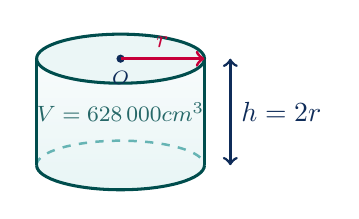
\begin{tikzpicture}[scale=0.82]
      \def\r{1.3}
      \def\h{1.65}
      % ផ្ទៃតួស៊ីឡាំង (Shading)
      \fill[top color=brandLightBlue!60, bottom color=brandTealBg] (-\r,0) -- (-\r,\h) arc(180:360:\r cm and 0.38cm) -- (\r,0) arc(0:-180:\r cm and 0.38cm);
      % បាតក្រោមផ្នែកខាងក្នុង (បន្ទាត់ដាច់ៗ)
      \draw[dashed, brandTeal!60, line width=0.9pt] (-\r,0) arc (180:0:\r cm and 0.38cm);
      % បាតក្រោមផ្នែកខាងមុខ
      \draw[brandDarkTeal, line width=1.1pt] (-\r,0) arc (180:360:\r cm and 0.38cm);
      % គែមឆ្វេង និងស្តាំ
      \draw[brandDarkTeal, line width=1.1pt] (-\r,0) -- (-\r,\h);
      \draw[brandDarkTeal, line width=1.1pt] (\r,0) -- (\r,\h);
      % បាតខាងលើ
      \fill[brandTealBg!85] (0,\h) ellipse (\r cm and 0.38cm);
      \draw[brandDarkTeal, line width=1.1pt] (0,\h) ellipse (\r cm and 0.38cm);
      % ផ្ចិត O និងកាំ r
      \fill[brandNavy] (0,\h) circle (1.8pt) node[below=1pt, font=\scriptsize\bfseries, color=brandNavy] {$O$};
      \draw[brandCrimson, line width=1.1pt, ->] (0,\h) -- (\r,\h);
      \node[above, font=\small\bfseries, color=brandCrimson] at (\r*0.5, \h+0.02) {$r$};
      % បន្ទាត់បង្ហាញកម្ពស់ h = 2r
      \draw[brandNavy, line width=1pt, <->] (\r+0.4, 0) -- (\r+0.4, \h);
      \node[right, font=\normalsize\bfseries, color=brandNavy] at (\r+0.42, \h*0.5) {$h = 2r$};
      % ស្លាកបង្ហាញមាឌខាងក្នុង
      \node[font=\footnotesize\bfseries, color=brandDarkTeal!85] at (0, \h*0.5) {$V = 628\,000\text{ cm}^3$};
    \end{tikzpicture}%
  }\par\vspace{5pt}

  % --- លំហាត់ ២៣ ---
  \exhead{23} \textbf{លំហាត់ពង្រឹងស្វ័យគុណ ៖}\par
  \khmodel{%
    \circnum{1} $2^{17} + 2^{17} = 2(2^{17}) = 2^{18}$ \quad
    \circnum{5} $2^{2x+3} = 2^{15} \implies x = 6$%
  }
  \textbf{ក. បង្ហាញសមភាព ៖}\par
  \coltwo{\circnum{1} $2^{17} + 2^{17} = 2^{18}$}{\circnum{2} $3^{15} + 3^{15} + 3^{15} = 3^{16}$}
  \coltwo{\circnum{3} $4^8 + 4^8 = 2^{17}$}{\circnum{4} $9^5 + 9^5 + 9^5 = 3^{11}$}\par\vspace{2pt}
  \textbf{ខ. រកតម្លៃ $x$ ៖}\par
  \coltwo{\circnum{5} $2^x \cdot 2^{x+3} = 8^5$}{\circnum{6} $3^x \cdot 3^{x+1} = 27^3$}
  \coltwo{\circnum{7} $\dfrac{2^{3x-1}}{2^{x+1}} = 16$}{\circnum{8} $4^{x+1} = 2^{3x-2}$}\par\vspace{2pt}
  \textbf{គ. គណនា និងប្រៀបធៀប ៖}\par
  \coltwo{\circnum{9} $A = \dfrac{2^{10} \cdot 3^8}{6^7}$}{\circnum{10} ប្រៀបធៀប $2^{30}$ និង $3^{20}$}

\end{multicols}

\vfill

% ៥. បដាពាក្យស្លោកខាងក្រោម (Bottom Motto Banner)
\begin{tcolorbox}[
  enhanced,
  colback=brandTealBg,
  colframe=brandNavy!30,
  arc=3.5pt,
  boxrule=0.7pt,
  top=3pt, bottom=3pt,
  center,
  halign=center
]
  \fontsize{9.5}{9.5}\selectfont\color{brandNavy}
  \textbf{\ding{228}\ \textit{Please don't stop and stop when you're done!} \ding{228}}
\end{tcolorbox}

\end{document}
